
\chapter{External Photon Conversion in sPHENIX Detector}
\label{app:external_conversion}

\section{Overview of External Conversion}

In heavy ion collision, precision of \ac{EMCal} measurements relies on the accurate reconstruction of photons originating from the primary collision vertex. However, before reaching the \ac{EMCal}, these photons must traverse the internal detector subsystems like \ac{MVTX}, \ac{INTT}, \ac{TPC} and the beryllium beam pipe. These subsystems and their mechanical support structures represent a significant material budget. Any photon traversing this material possess a non-negligible probability of undergoing pair production ($\gamma \rightarrow e^+ + e^-$) before interacting with the \ac{EMCal}. In addition, the \ac{sPHENIX} detector operates within a 1.4~T (Tesla) magnetic field which deflects those converted $e^+ e^-$ pairs significantly. Such deflection, sometimes, can create two distinct and well separated \ac{EMCal} clusters. Since, external conversion affects the clusters, they should be corrected accounted for our study of neutral mesons.

\section{Neutral Meson Reconstruction}

As we analyzed neutral meson via two photon decay mode, we expect two \ac{EMCal} clusters: one for each photon. As external conversion of photon creates more than two clusters, thus, introduces a systematic effect in our analysis. The most robust way of analyzing external conversion utilized the track related information. Since such information were not available for our data, we estimated the external conversion via the number of \ac{EMCal} clusters in simulation. For this, we simulated single meson decay per event and pass through the full \textbf{GEANT4} description of the \ac{sPHENIX} detector. In reconstructed data, if there exists more than two clusters, those meson certainly have undergone external conversion. If only one cluster is present, we ignore that meson in our analysis, as they could be associated with efficiency and not external conversion.

The situation becomes nontrivial when exactly two clusters were present. To study this subtle situation, we developed a conservative method to identify if either of the photon from parent meson have converted after interacting with detector. First, we matched each cluster to one of the two truth photons by choosing the closest in $\Delta R$. Such matching must be unique in a sense there must be one photon to one cluster matching. Additional criteria was that every matches must be sufficiently close in angular distance ($\Delta R \leq 0.5$) and energy asymmetry between photon and cluster must be $E_{\alpha} \leq 0.6$. When any of these criteria was not satisfied, the parent meson was considered as suffering from external conversion. 

 

\begin{figure}[H]
  \centering
  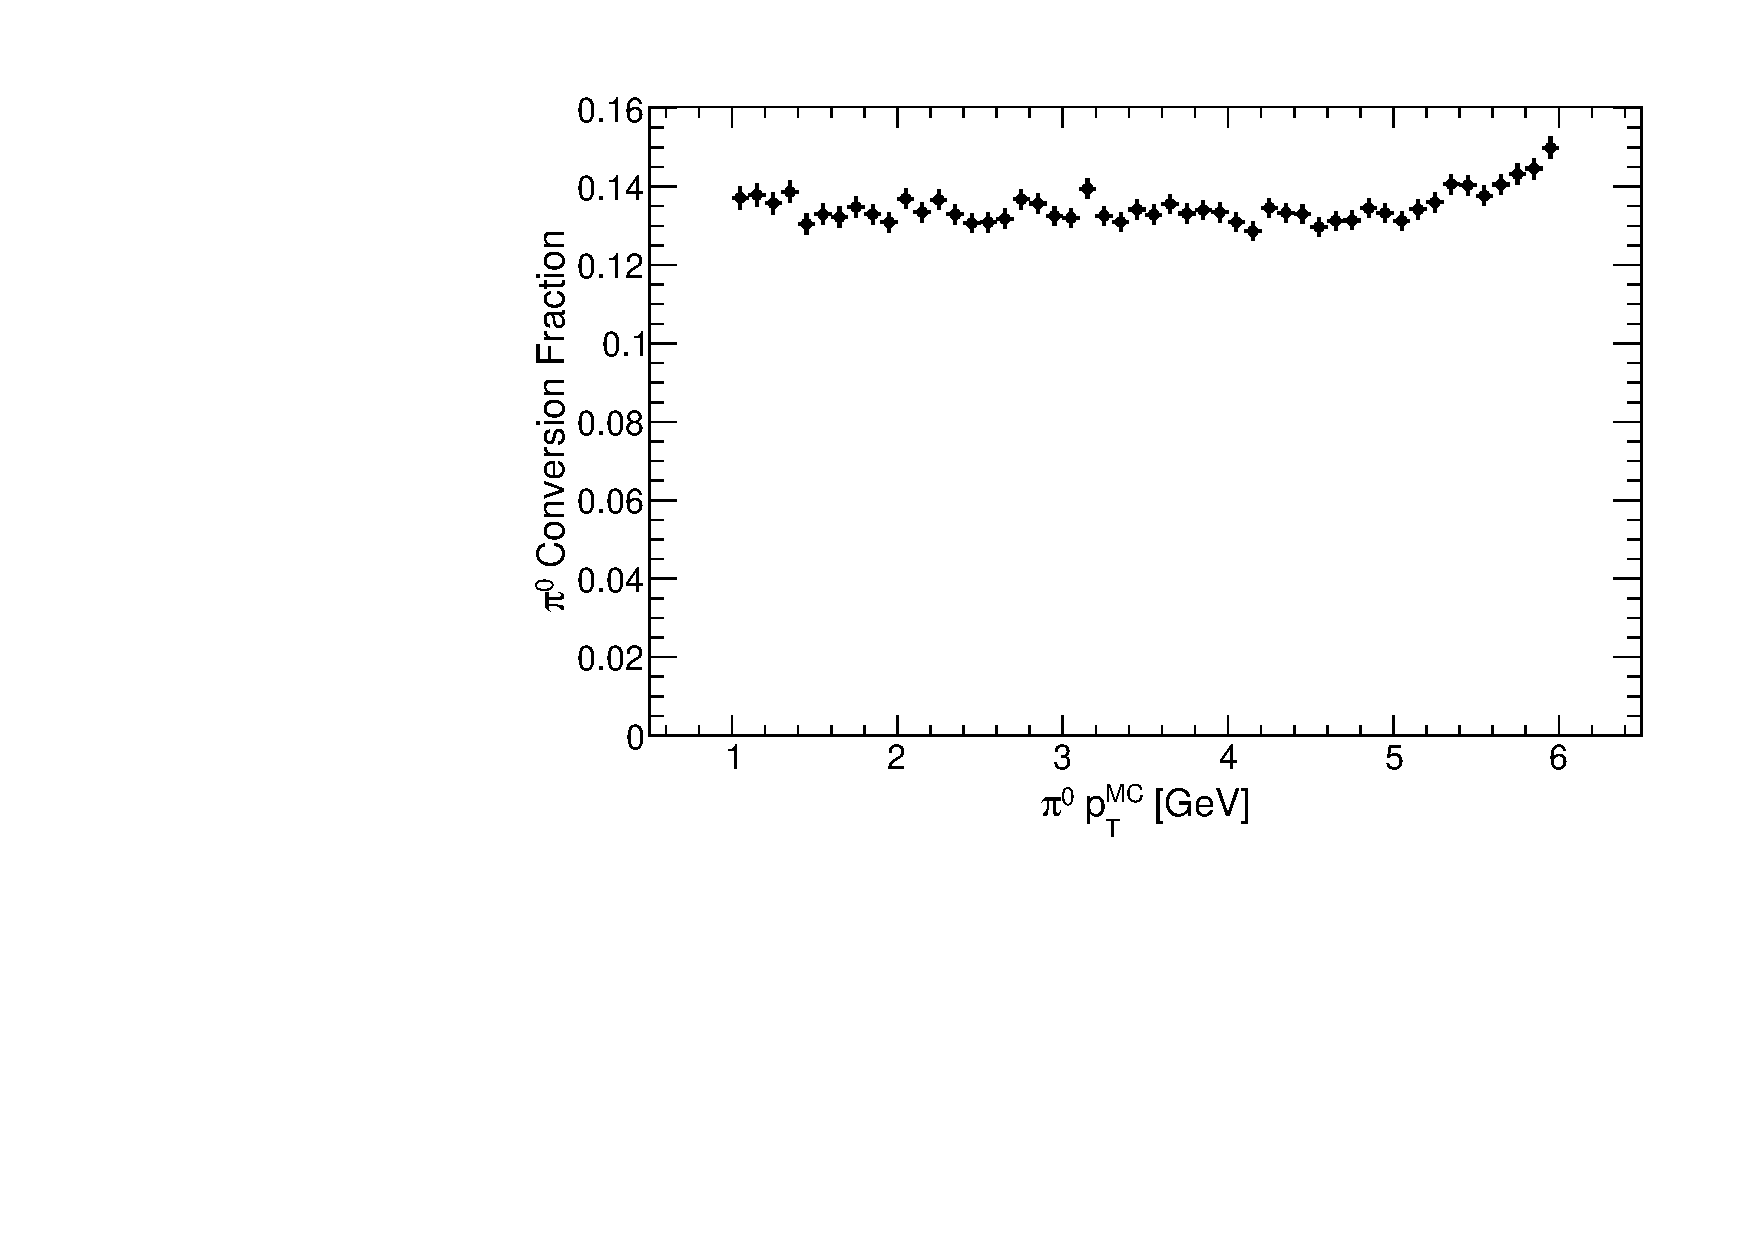
\includegraphics[width=0.95\textwidth,
    alt={Plot of the fraction of simulated neutral pions with at least one
         converted photon versus generated transverse momentum from 1 to
         6 GeV. The fraction is nearly constant at about 0.13 to
         0.14.}]{Images/App/frac_pi0_conversion.pdf}
  
  \caption{Study of external photon conversions as a function of transverse momentum ($p_T$) for $\pi^0 \rightarrow \gamma\gamma$, where at least one of the photon gets converted before being detected in \ac{EMCal}.}

  \label{fig:pi0_conver}
\end{figure}


\begin{figure}[H]
  \centering
  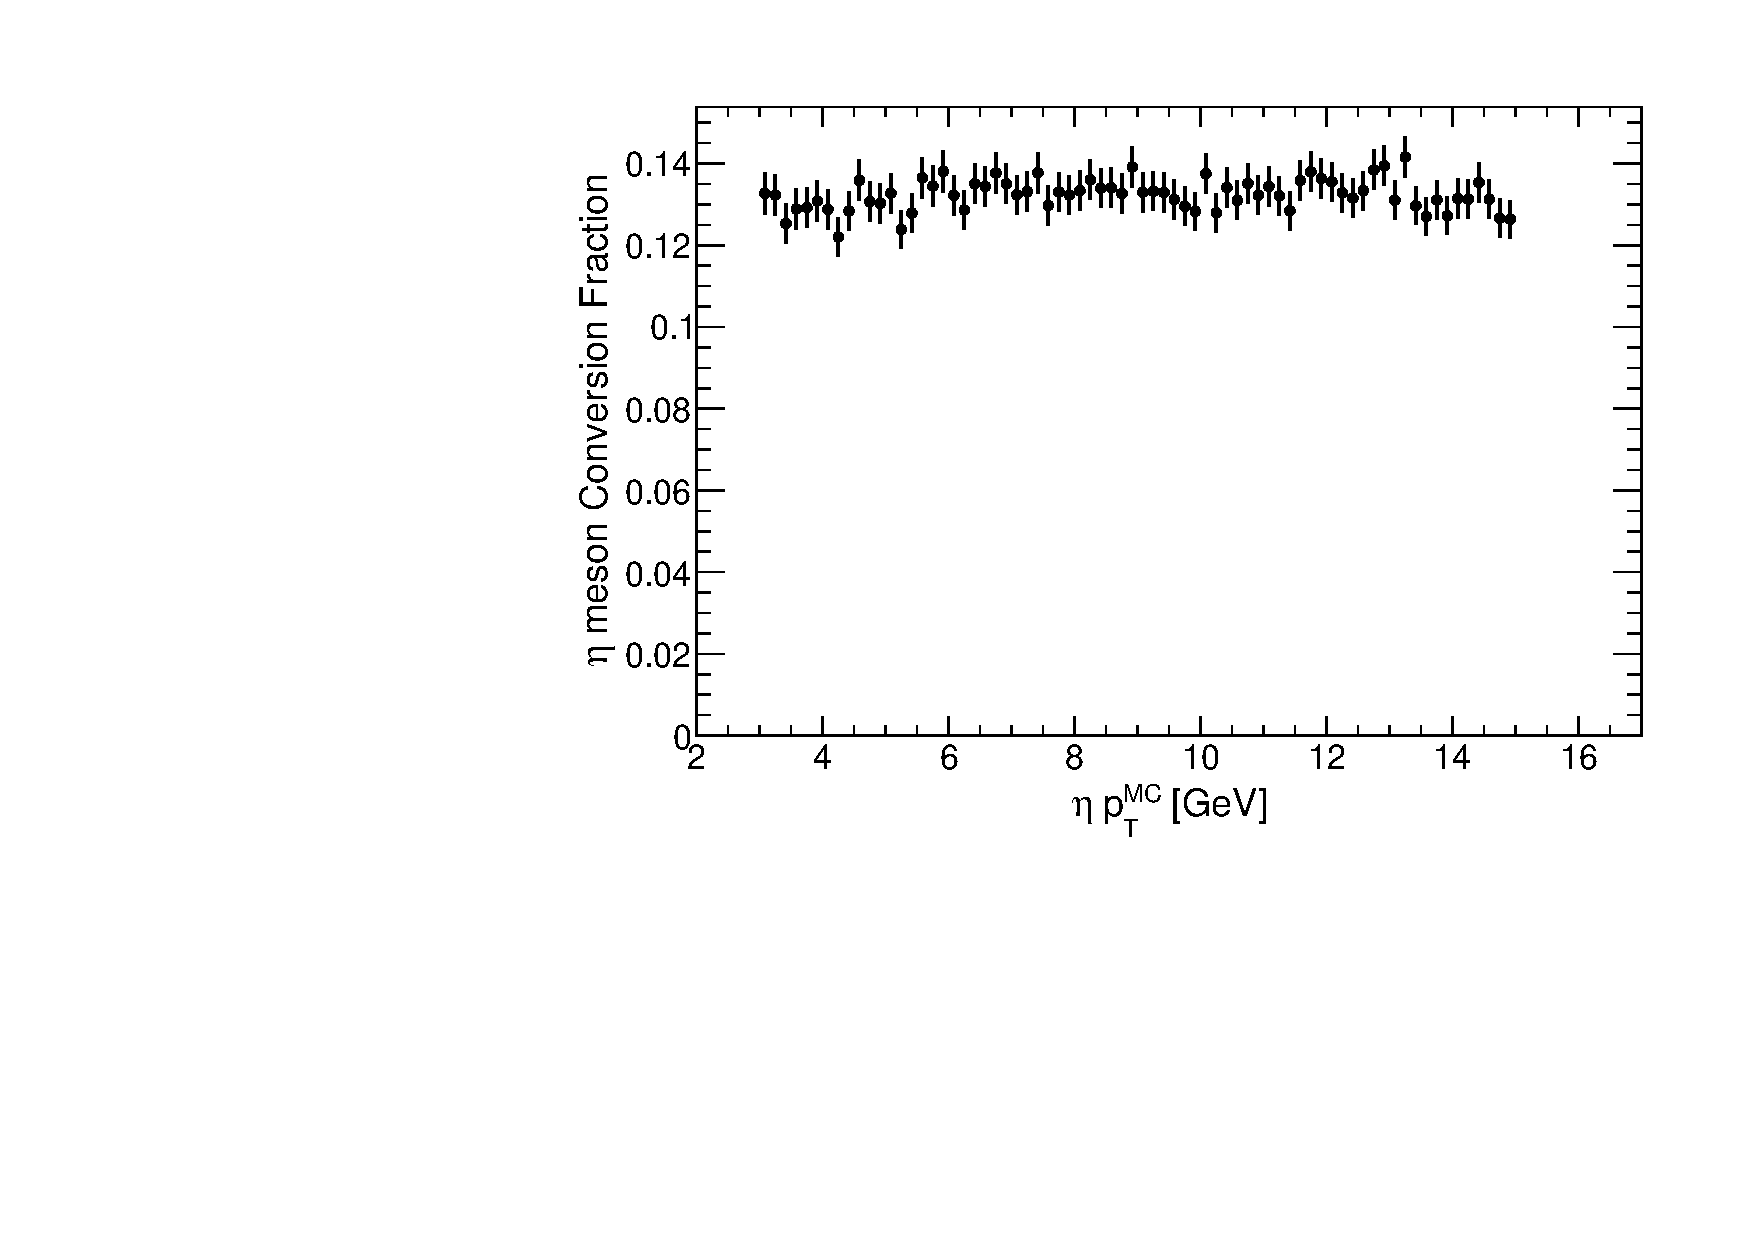
\includegraphics[width=0.95\textwidth,
    alt={Plot of the fraction of simulated eta mesons with at least one
         converted photon versus generated transverse momentum from 3 to
         15 GeV. The fraction is nearly constant at about
         0.13.}]{Images/App/frac_eta_meson_conversion.pdf}
  \caption{Study of external photon conversions as a function of transverse momentum ($p_T$) for $\eta$ meson decaying to two photons. Here, the conversion fraction reflects the probability that at least one of the decayed photon undergoes conversion.}

  \label{fig:eta_conver}
\end{figure}



The figure \ref{fig:pi0_conver} and figure \ref{fig:eta_conver} suggest approximately 13 - 14 \% of both $\pi^0$ and $\eta$ meson was affected by external conversion which is significant for our study. As this study was a simple conservative estimate, this percentage could be slightly different on using more robust analysis. This conclusion give us a motivation to use side-band fitting method as primary standard method for background estimation.
 
The external photon conversion was fully modeled within the detector simulation framework, and its impact was systematically propagated while calculating detector efficiency. Therefore, no independent or supplementary study was required to account for this effect for the scope of this study.

